\documentclass[a4paper, 12pt]{article}

\usepackage[english, russian]{babel}
\usepackage[utf8]{inputenc}
\usepackage[T2A]{fontenc}
\usepackage{verbatim}
\usepackage{amsmath, amsthm}
\usepackage{geometry}
\usepackage{titlesec}
\usepackage{graphicx}
\usepackage{enumitem}

\geometry{
	a4paper,
	top=1cm,
	bottom=1cm}

\titlespacing*{\section}{0mm}{0mm}{0mm}
\titlespacing*{\subsection}{0mm}{0mm}{2mm}

\makeatletter
\AddEnumerateCounter{\asbuk}{\russian@alph}{щ}
\makeatother

\begin{document}
	\clearpage
	\pagestyle{empty}
	\section*{$1$ тур}
	\subsection*{Математика}
	Имеется $101$ монета, одна из которых фальшивая, отличающаяся по весу от настоящих. Можно ли за $2$ взвешивания на чашечных весах понять, легче или тяжелее фальшивая монета, чем настоящие?
	\subsection*{Физика}
	 Поезд проезжает треть маршрута Самара-Нижний Новгород ($174$ км) за $3$ часа, после этого понижает свою скорость до $29$ км/ч. Найдите среднюю скорость поезда на всём пути. Ответ округлите до целых.
	 \subsection*{Информатика}
	 Использую логические И, ИЛИ и отрицание составьте формулу $F$ со следующей таблицей истинности.
	 \begin{center}
	 		 \begin{tabular}{|c|c|c|c|}
	 		\hline
	 		X & Y & Z & F \\
	 		\hline
	 		0 & 0 & 0 & 0 \\
	 		\hline
	 		0 & 0 & 1 & 1 \\
	 		\hline
	 		0 & 1 & 0 & 1 \\
	 		\hline
	 		0 & 1 & 1 & 0 \\
	 		\hline
	 		1 & 0 & 0 & 1 \\
	 		\hline
	 		1 & 0 & 1 & 0 \\
	 		\hline
	 		1 & 1 & 0 & 0 \\
	 		\hline
	 		1 & 1 & 1 & 1 \\
	 		\hline
	 	\end{tabular}
	 \end{center}
	 \subsection*{Биология}
	 Как вы знаете, бывают сухопутные ежи, также называемые настоящими, и морские ежи. Однако до сих пор не находили летающих ежей. Как вы думаете, какие особенности строения тела обыкновенного ежа не позволяют ему освоить воздушное пространство?
	 \subsection*{Химия}
	 Составьте цепочку: 
	 \[\text{А}\to\text{Б}\to\text{В}\to\text{Г}\to\text{Д}\to\text{Е}\to\text{Ё}\to\text{Ж}\]
	 \begin{itemize}
	 	\item[А] --- элемент, проявляющий единственную степень окисления, равную $-1$
	 	\item[Б] --- номер группы элемента А
	 	\item[В] ---  элемент, имеющий Б протонов в ядре
	 	\item[Г] --- номер группы элемента В
	 	\item[Д] --- галоген периода номер Г
	 	\item[Е] --- молярная масса элемента Д (с точностью до целых)
	 	\item[Ё]$=(\text{Е} - \text{З}\cdot\text{Г})/\text{Б}$
	 	\item[Ж] --- элемент с молярной массой Ё
	 \end{itemize}
 	 \subsection*{Гуманитарные науки}
 	 Перечислите пять известных вам личностей по имени Александр, прославившихся в истории прошлых веков (государственные и общественные деятели, ученые, деятели культуры и т.д.). Кратко изложите, чем именно они вписали свое имя в историю. Приведите как минимум два достижения (открытие, произведение, реформа и т.д.)
 	 
	 \newpage
	 \clearpage
	 \pagestyle{empty}
	 \section*{$2$ тур}
	 \subsection*{Математика}
	 Найдите наименьшее натуральное n, при котором число $A = n^3 + 12n^2 + 15n + 180$ делится на $23$.
	 \subsection*{Физика}
	 В железный котёл массой $5$ кг налита вода массой $10$ кг. Какое количество теплоты нужно передать котлу с водой для изменения температуры в системе от $10$ до $100^\circ$C? Удельная теплоемкость железа $460$ Дж/кг$^\circ$C, удельная теплоемкость воды $4200$ Дж/(кг $^\circ$C). Ответ укажите в кДж.
	 \subsection*{Информатика}
	 На прямой дано множество отрезков. Необходимо найти максимальный размер множества непересекающихся отрезков.
	 \subsection*{Биологиия}
	 Учитель показал Вове две фотографии разных сосудов. Помогите ему ответить на вопросы:
	 \begin{enumerate}
	 \item На какой фотографии изображена вена, а на какой артерия? Почему вы так решили?
	 \item В каких сосудах больше давление? А площадь сечения? Куда и какая кровь по ним течет?
	 \item Из каких оболочек состоит стенка сосудов? Почему их толщина различается?
	 \item За счет чего кровь течет по венам? 
	 \end{enumerate}
	 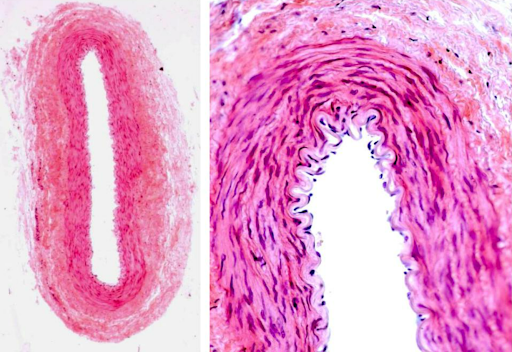
\includegraphics[scale=0.7]{1}\\
	 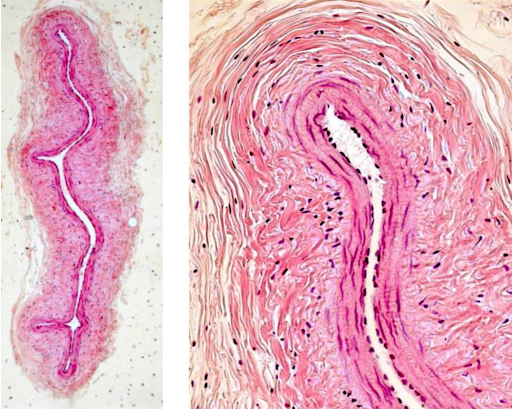
\includegraphics[scale=0.7]{2}
	 \subsection*{Химия}
	 Рассчитайте молярную массу двух соединений, имеющих формулы:
	 \begin{center}
	 	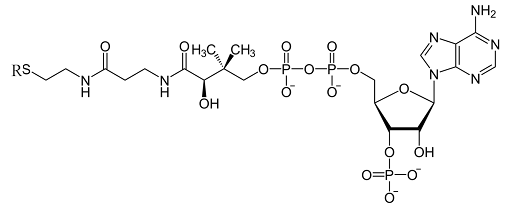
\includegraphics[width=\textwidth]{4}
	 \end{center}
 	 \begin{enumerate}[label=\asbuk*), ref=\asbuk*]
 	 	\item $R=H$
 	 	\item $R=$
 	 	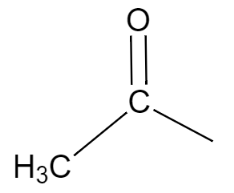
\includegraphics[scale=0.3, trim=5mm 30mm 0 0]{5}
 	 \end{enumerate}
  \hspace*{1pt}
  	 \subsection*{Гуманитарные науки}
  	 Прочтите слово приезд.
  	 
  	 \noindent \textit{Задание.} Определите, сколько раз каждый звук этого слова встречается в следующей фразе: жили-были старик со старухой.
  	 
	 \newpage
	 \clearpage
	 \pagestyle{empty}
	 \section*{$3$ тур}
	 \subsection*{Математика}
	 Гидры состоят из голов и шей (каждая шея соединяет ровно две головы). Одним ударом меча можно снести все шеи, выходящие из какой-то головы $A$ гидры. Но при этом из головы $A$ мгновенно вырастает по одной шее во все головы, с которыми $A$ не была соединена. Геракл побеждает гидру, если ему удастся разрубить её на две несвязанные шеями части. Найдите наименьшее $N$, при котором Геракл сможет победить любую стошеюю гидру, нанеся не более чем $N$ ударов.
	 \subsection*{Физика}
	 В схеме, изображенной на рисунке в начальный момент все пространство между обкладками плоского конденсатора полностью заполнено пластиной с диэлектрической проницаемостью $\varepsilon$. Емкость такого конденсатора $C_2$. Пластину начинают медленно с постоянной скоростью выдвигать из конденсатора. Через некоторое время на конденсаторе емкостью $C_1$ устанавливается постоянное напряжение $U$ с положительным зарядом на левой обкладке. Для этого установившегося режима определить: 
	 \begin{enumerate}
	 	\item ток через батарею с ЭДС $\varepsilon_1$;
	 	\item скорость перемещения пластины.
	 \end{enumerate}
	 Размер обкладок конденсатора с начальной емкостью $C_2$ в направлении перемещения пластины равен $L$. Внутренними сопротивлениями батарей пренебречь. Величины $\varepsilon, I, L, \varepsilon_1, \varepsilon_2, C_1$ и $R$ считать известными. Обкладки конденсатора и пластина имеют прямоугольную форму. 
	 \begin{center}
	 	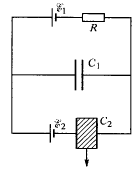
\includegraphics{3}
	 \end{center}
 \subsection*{Информаткиа}
 Удалось: получить: несколько зашифрованных слов, которые в незашифрованном виде были лекосикографически отсортированы. Эти слова состоят из прописных букв латинского алфавита. Ваша задача состоит в том, чтобы вы восстановили шифрующую строку. Известно, что входной словарь состоит из подряд идущих букв латинского алфавита и известна его мощность. Например, если мощность алфавита равна $5$ и шифрующая строка $BAEDC$, то все символы $A$ преобразуются в $B$, $B$ --- в $A$, $C$ --- в $E$, $D$ останется неизменным, $C$ --- в $E$
 
 \begin{tabular}{|l|}
 	\hline
 	Вход \\
 	\hline
 	5 \\
 	20 \\
 	DDCDA\\ 
 	DDADE \\
 	DDECE \\
 	DCEAC \\
 	DCEAA \\
 	DBADA \\
 	DBACB \\
 	ADCCE \\
 	ACCDE \\
 	ACCDB \\
 	ABCDA \\
 	ABEDA \\
 	EDCDA \\
 	ECCDB \\
 	ECADE \\
 	ECAAE \\
 	ECEDE \\
 	EBCDE
 	\\
 	\hline
 \end{tabular}
 \subsection*{Биология} 
 В $1928$ году ученый Ф. Гриффит опубликовал результаты своего эксперимента, в котором он заражал мышей штаммами пневмококков, вызывающих пневмонию и у человека, и у мышей. Колонии, которые образуют капсулу, высоко вирулентны и при культивировании имеют гладкую поверхность. Они называются $S$-формами, а мутантные $R$-формы утратили способность к образованию капсулы и не имеют вирулентности. У Гриффита было $3$ контрольных группы: мыши, зараженные $S$-вирулентной формой, мыши, зараженные $R$-формой и мыши, зараженные убитыми пневмококками $S$-формы. А также одна опытная "--- мыши, зараженные смесью убитых $S$-форм и живых $R$-форм. Мыши опытной группы скончались :( Предположите, что случилось с $3$-мя контрольными группами. Опишите и назовите процесс, происходящий с пневмококками опытной группы. Зачем в этом эксперименте каждый из трёх контролей?
 \subsection*{Химия}
 Образец минерала с планеты КВАЧ, содержит $13,36\%$ алюминия, $37,12\%$ мышьяка и $47,52\%$ кислорода. Оставшиеся проценты принадлежат элементу, имеющему непостоянную  прописку  в таблице Менделеева. Определите формулу минерала, дайте ему химическое название,и определите к какому классу веществ он относится?
 Рассчитайте сколько литров воды потребуется, чтобы растворить $1$г этого кристаллогидрата, если его ПР$=3,6\cdot10^{-24}$
 \subsection*{Гуманитарные науки}
 \textit{Часть 1.}\\
 Что значит «гуманитарная» наука? Чем гуманитарные науки отличаются от социальных? Подготовьте развёрнутый ответ и определение.
 
 \noindent\textit{Часть 2.} \\
 Придумайте три контрпримера для своего определения. Является ли существование этих контрпримеров проблемой для вашего определения? Если да, придумайте как модифицировать своё определение, если нет, объясните почему наличие контрпримеров не является проблемой.
\end{document}